\subsection{Applications}\label{sec:apps}

One of the appeals of this approximate patch-based approach
is that it naturally lends itself to applications. In this
section we describe methods to use our database for
two applications - duplicate detection and similar image retrieval.

\subsubsection{Duplicate Detection}\label{sec:dups}

Encoding images as pointers to a collection of patches provides the ability to quickly spot images that contain large overlapping regions (composed of the same patches). In the extreme case, if multiple images point to the same set of patches, then we know these images are duplicates. Duplicates are a big problem in big computer vision datasets because they occur frequently and are hard to manually remove. They occur frequently (sometimes up to $10\%$ of the time) because these datasets are automatically scraped from the internet, where the same image can occur under separate identifiers (on different websites, copied and uploaded by different users, etc.). The SUN database \cite{SUN} used in this paper is no exception.

Duplicates are difficult to detect because not all duplicates are pixel-wise identical: the same image encoded using different standards or sized to different dimensions (even when resized to the same dimension later) will look almost identical to the human eye, but will contain different pixel values. Our patch distance metric is forgiving to perturbation at the pixel-level as long as the patch is overall similar to another patch (see sec.\ref{sec:simthresh}). If multiple images map to the same set of patches that means that the corresponding patches in those images are within a distance threshold of each other (upper-bounded by $2T$). If multiple images map to all of the same patches, then we have good guarantees that the images are near-duplicates. Otherwise, the probability that every single patch matched would be low (i.e. low that two images are similar locally, for multiple local locations - as many locations as patches).

We can use these properties to spot duplicates in our database on-the-fly. For instance, when an image is added to the database, we can measure how many new patches the image contributed to the patch dictionary (because similar-enough patches could not be found), and how much of the image was mapped to pre-existing dictionary patches. When an image is reconstructed fully from the dictionary patches, and the patches it is reconstructed from all come from a single other image in the database, we know that the newly-added image is a duplicate. This is depicted in fig. \ref{fig:dups}.

By the same logic, similar images are those that overlap in terms of the patches they share in common. We can easily compare the two patch pointer vectors of two images to check their overlap. We can check if this overlap corresponds to patches clustered together in the images (for instance, when only some local region of the images matches, like when they share an object). We can thus discover images that have different degrees of overlap with other images.

 \begin{figure}
\hspace{-8mm}
%\centering
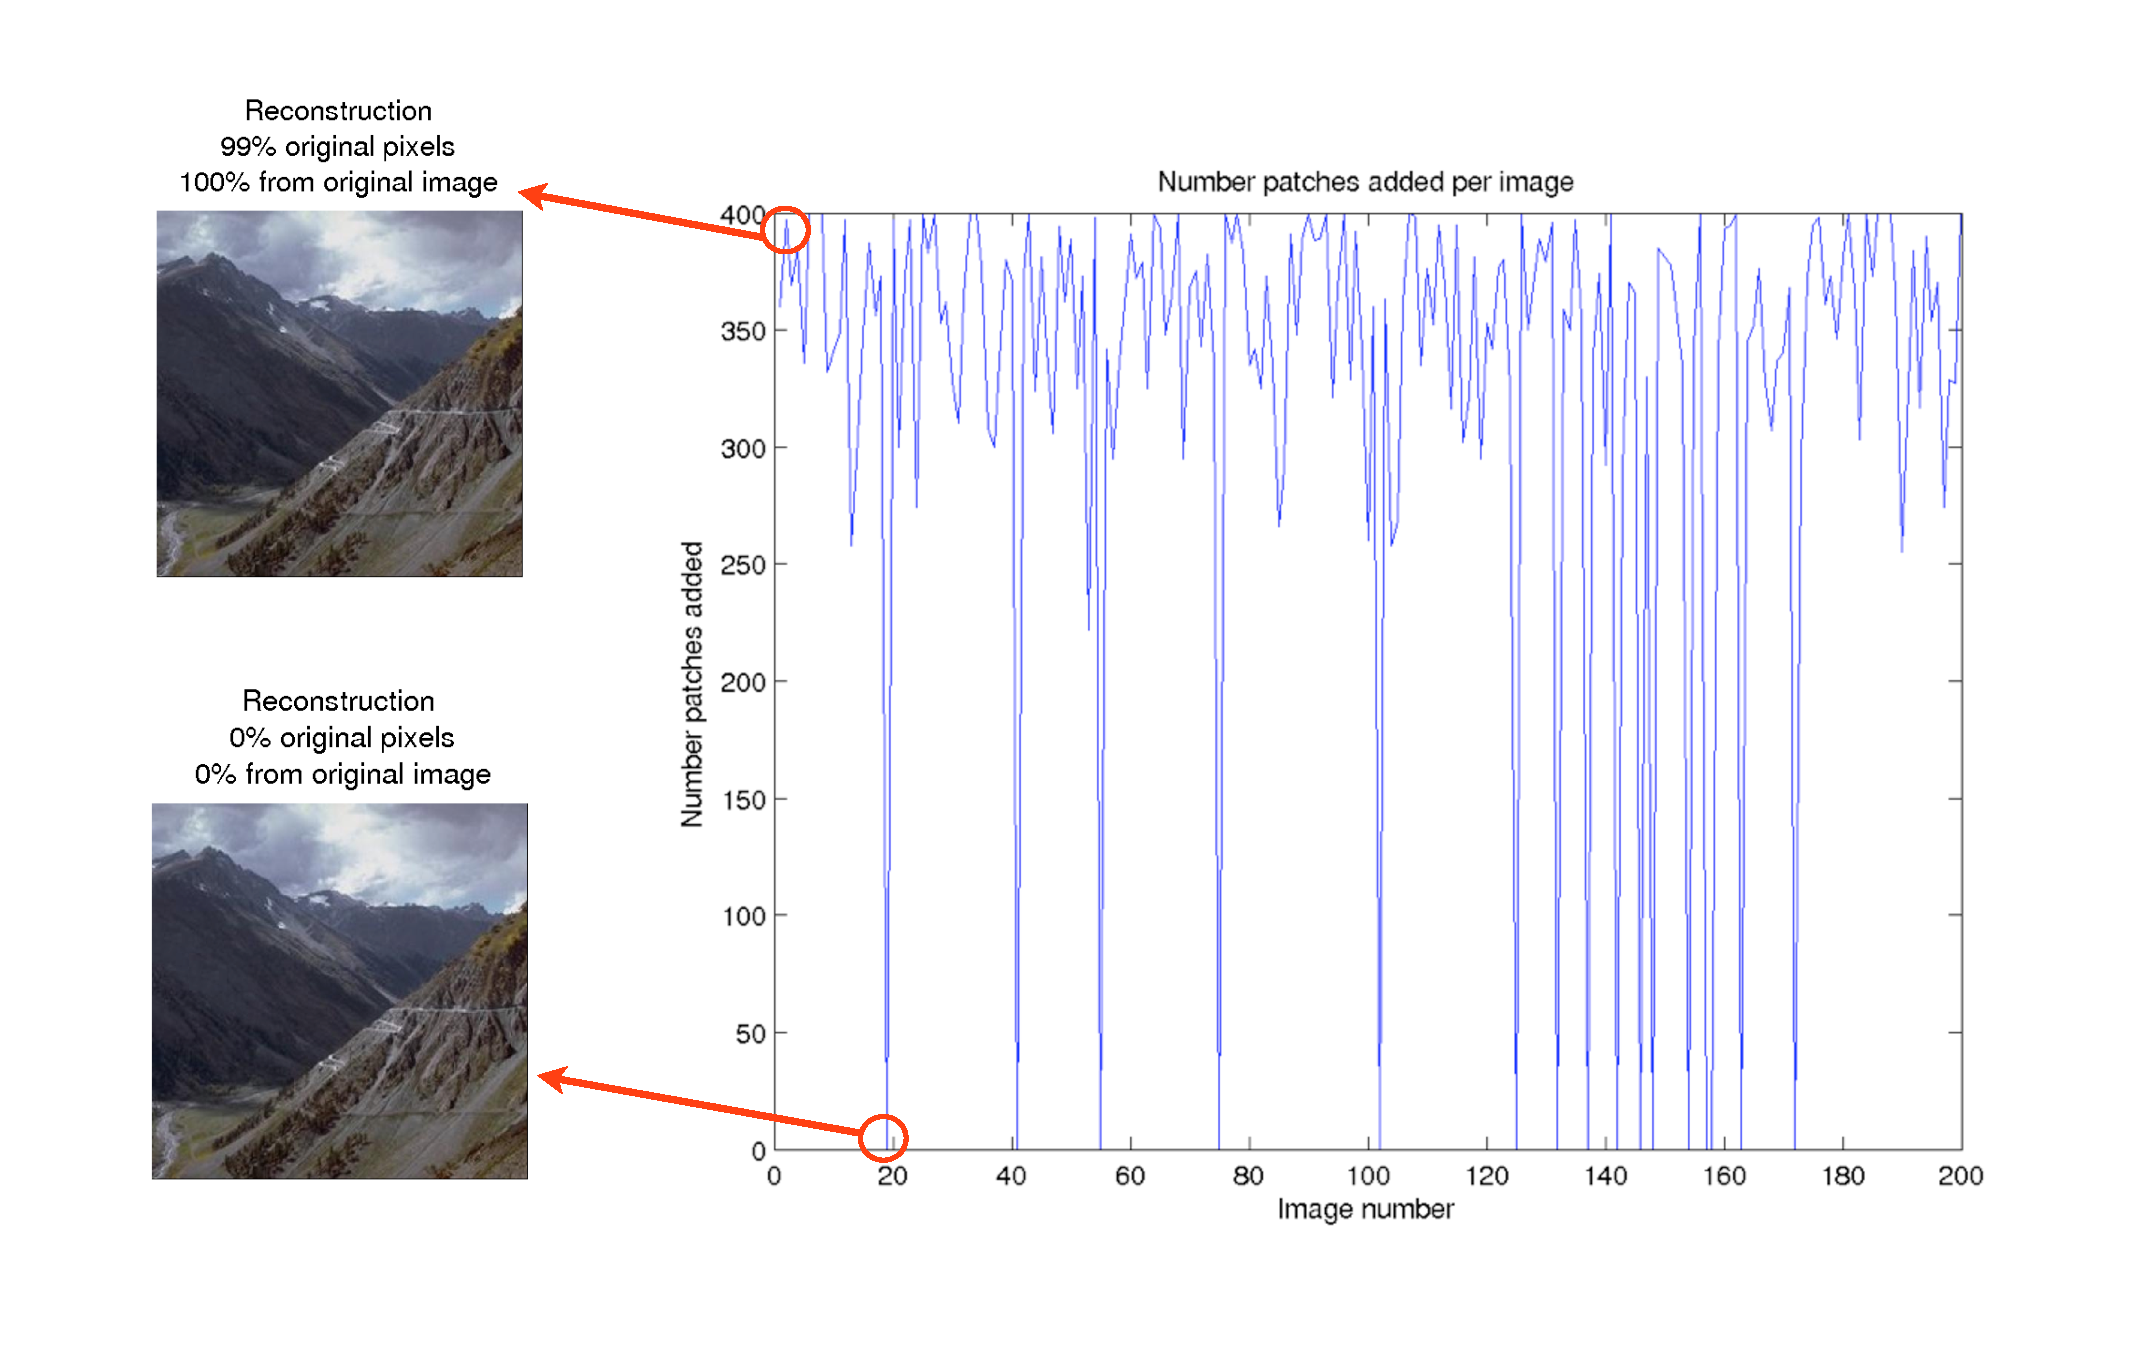
\includegraphics[width=1.2\linewidth]{Figures/dupDetection.pdf}
\caption{This is an example of the first 200 consecutive insertion queries to an empty database: for each image inserted, we can measure how many new patches were added to the patch dictionary (out of 400 patches in the image). When we see that this number spikes down to 0 we know that the image has been fully reconstructed from patches from other images. We can check if all those patches came from a single other image. If that is the case, we know we have a duplicate or near-duplicate image. }
\label{fig:dups}
\end{figure}

\subsubsection{Photomosaics}\label{sec:photo}

One interesting (and somewhat whimsical) application of our system is in the automated fabrication of photomosaics from images.  A photomosaic \footnote{See, for example, \url{http://en.wikipedia.org/wiki/Photographic_mosaic}.} is an image which is created by partitioning a pre-existing 2-D piece of artwork into small, equally sized rectangles.  Each of these rectangles is then replaced with a small image which approximates the original color and texture of the rectangle, keeping the overall artwork recognizable.  Thus, the final result is an image composed of hundreds of smaller images.

Our system can be directly applied to the synthesis of such images, with a few very small modifications.  First, instead of determining which patches to store based on our previous dictionary and image collection, we a priori store a selected input image set as our patch dictionary, but scaled to "patch size."  For demonstration purposes, we created our patch dictionary by scaling down and storing the entire SUN database.  In order to create the photomosaic, we first choose and store a target image we would like to transform.  In storing the image, we, as usual, split the image into patches, and for each patch perform a nearest neighbor search.  However, in this case, if no patch already exists in the hashed bin, we expand our nearest neighbor search to more bins until we find a bin with at least one patch, and choose the most similar one.  During this step, we \emph{never} store patches; we always map the patch to one already in the dictionary.  The mapping output by this process results in a photomosaic.

We demonstrate this process on a 1600x1200 image of the Stata Center at MIT, using 25x25 rectangular patches.  We show the original image and reconstruction in figure \ref{fig:stata}.


